\documentclass{article}

% if you need to pass options to natbib, use, e.g.:
% \PassOptionsToPackage{numbers, compress}{natbib}
% before loading nips_2016
%
% to avoid loading the natbib package, add option nonatbib:
\usepackage[nonatbib]{nips_2016}

%\usepackage{nips_2016}

% to compile a camera-ready version, add the [final] option, e.g.:
% \usepackage[final]{nips_2016}

\usepackage[utf8]{inputenc} % allow utf-8 input
\usepackage[T1]{fontenc}    % use 8-bit T1 fonts
%\usepackage{hyperref}       % hyperlinks
\usepackage{url}            % simple URL typesetting
\usepackage{booktabs}       % professional-quality tables
\usepackage{amsfonts}       % blackboard math symbols
\usepackage{nicefrac}       % compact symbols for 1/2, etc.
\usepackage{microtype}      % microtypography
\usepackage{amsmath}
\usepackage{mathtools}
\usepackage{fancyvrb}
\usepackage{multirow}
\usepackage{color}


% HT http://tex.stackexchange.com/a/151987/41154
\DeclarePairedDelimiterX{\infdivx}[2]{(}{)}{%
  #1\;\delimsize\|\;#2%
}
\newcommand{\dkl}{D_\mathrm{KL}\infdivx}

\usepackage{listings}
\definecolor{lightgray}{rgb}{.9,.9,.9}
\definecolor{darkgray}{rgb}{.4,.4,.4}
\definecolor{purple}{rgb}{0.65, 0.12, 0.82}
\definecolor{orange}{rgb}{1,0.5,0}

\definecolor{Red}{RGB}{255,0,0}
\newcommand{\red}[1]{\textcolor{Red}{#1}}
\definecolor{Green}{RGB}{10,200,100}
\definecolor{Blue}{RGB}{10,100,200}
\newcommand{\ndg}[1]{\textcolor{Green}{[ndg: #1]}}
\newcommand{\mht}[1]{\textcolor{Blue}{[mht: #1]}}
\newcommand{\lou}[1]{\textcolor{orange}{[lou: #1]}}

% casual outlining font
\newcommand{\cas}[1]{ \textsf{\color{darkgray} \scriptsize #1} }

\lstdefinelanguage{JavaScript}{
  keywords={typeof, new, true, false, catch, function, return, null, catch, switch, var, if, in, while, do, else, case, break},
  keywordstyle=\color{blue}\bfseries,
  ndkeywords={class, export, boolean, throw, implements, import, this},
  ndkeywordstyle=\color{darkgray}\bfseries,
  identifierstyle=\color{black},
  sensitive=false,
  comment=[l]{//},
  morecomment=[s]{/*}{*/},
  commentstyle=\color{purple}\ttfamily,
  stringstyle=\color{red}\ttfamily,
  morestring=[b]',
  morestring=[b]"
}

\lstset{
   language=JavaScript,
   backgroundcolor=\color{white},
   extendedchars=true,
   basicstyle=\footnotesize\ttfamily,
   showstringspaces=false,
   showspaces=false,
   numbers=none,
   numberstyle=\footnotesize,
   numbersep=9pt,
   tabsize=2,
   breaklines=true,
   showtabs=false,
   captionpos=b
}



\usepackage[ruled,vlined]{algorithm2e}

\newcommand{\ud}{\,\mathrm{d}}
\DeclareMathOperator*{\argmax}{arg\,max}


\title{Practical optimal experiment design for psychology}

% The \author macro works with any number of authors. There are two
% commands used to separate the names and addresses of multiple
% authors: \And and \AND.
%
% Using \And between authors leaves it to LaTeX to determine where to
% break the lines. Using \AND forces a line break at that point. So,
% if LaTeX puts 3 of 4 authors names on the first line, and the last
% on the second line, try using \AND instead of \And before the third
% author name.

\author{
  David S.~Hippocampus\thanks{Use footnote for providing further
    information about author (webpage, alternative
    address)---\emph{not} for acknowledging funding agencies.} \\
  Department of Computer Science\\
  Cranberry-Lemon University\\
  Pittsburgh, PA 15213 \\
  \texttt{hippo@cs.cranberry-lemon.edu} \\
  %% examples of more authors
  %% \And
  %% Coauthor \\
  %% Affiliation \\
  %% Address \\
  %% \texttt{email} \\
  %% \AND
  %% Coauthor \\
  %% Affiliation \\
  %% Address \\
  %% \texttt{email} \\
  %% \And
  %% Coauthor \\
  %% Affiliation \\
  %% Address \\
  %% \texttt{email} \\
  %% \And
  %% Coauthor \\
  %% Affiliation \\
  %% Address \\
  %% \texttt{email} \\
}

\begin{document}
% \nipsfinalcopy is no longer used

\maketitle

\begin{abstract}
todo
\end{abstract}

\section{Introduction}
\ndg{Doing the standard, active learning thing with probabilistic programs. }

Designing scientific experiments is hard.
Scientists must have hypotheses and reason over a potentially large space of possible experiments.
Studying human behavior has additional complications.
Human data is noisy and sensitive to dependent measure of the task.
Further, human data is expensive and one must balance expected statistical power with the constraints of a limited budget to decide on the number of participants to run.

Formal models of psychological phenomena alleviate some of these issues.
Models make explicit hypotheses about observed data, and thus make it easier (or in some cases, possible) to explore the implications of a set of ideas.
However, exploring models can be time-consuming and searching through a large space of possible experiments is still largely driven by the scientist's intuition.
This need not be the case: If both the set of hypotheses and the space of experiments are explicit, then we can partially \emph{automate} experiment design as a sort of active learning problem, searching for experiments that maximally update our beliefs about a scientific question.

We present a general, principled, and turnkey approach to designing experiments that uses a Bayesian approach to find experiments that best distinguish competing hypotheses.
The framework is implemented in a \emph{probabilistic programming language} (PPL).
PPLs are a convenient way to represent explicit hypotheses about the data.
We show how optimal experiment design (OED) can be streamlined into a scientist's workflow by instantiating it in a user-friendly PPL in which formal hypotheses can already be expressed.
This is a crucial step in making a practical OED system: Once you're using a PPL to formalize your hypotheses, OED comes for free.
%\lou{as explained, this doesn't seem so crucial to me.}

%Though the framework is Bayesian, it is not directly related to Bayesian models of cognition; rather, it can be applied to any instance in which the scientist has a formal model of the data generating process (including, Bayesian models of cognition).

We are not the first to attempt to develop a framework for optimal experiments in psychology.
Previous attempts \lou{citations?}, however, suffer from a number of pragmatic issues, including ad-hoc optimization criteria, lack of an established pipeline, and failure to accommodate common worries in psychology experiments (e.g., dealing with noisy responses, determining sample sizes, and selecting dependent measures or linking functions).
% Taken together, these issues put the burden on researchers to have sufficient expertise to adapt the OED system to their specific problem and require researchers to develop their own system for writing formal psychological models and the OED optimization engine.

In this paper, we resolve these issues using a Bayesian model selection framework implemented in a practical modeling system.
We apply this framework to two case studies: perceptions of subjective randomness and category learning.
The first case study highlights the details of application for a simple space of experiments.
The second study applies OED to a more realistic space of possible experiments and validates our theoretical analysis by running the optimal experiment.
Our general system opens a number of rich areas for future development, which we explore in the discussion.

%We conclude by highlighting the generality of the approach and areas of future work.
%\ndg{all the parts are here. needs smoothing. make it clearer that using PPL to represent hypotheses is a key step in making the system practical.}

%    \begin{itemize}
%        \item It is difficult to discriminate models of psychological processes
%        \item Experiments are expensive
%        \item We present a general, turn-key approach to design experiments that best disambiguate competing models using a Bayesian framework
%        \item This technique is not directly related to Bayesian models of cognition. It can be used on any (formal / probabilistic) model, including Bayesian models of cognition
%        \item Despite the previous attempts in this field, there are a number of pragmatic issues that make it difficult to readily apply OED techniques for psychology, including:
%        \begin{itemize}
%            \item A variety of proposed optimization criteria, which puts the burden on researchers to have sufficient expertise to select the appropriate approach
%            \item A lack of an established pipeline, requiring researchers to develop a language to formalize psychological models and write an OED optimization engine
%            \item A lack of analysis in dealing with practical experimental concerns such as:
%                \begin{itemize}
%                    \item Noisy responses from participants
%                    \item The ideal number of participants for a study
%                    \item The ambiguity of linking functions of dependent measures
%                \end{itemize}
%        \end{itemize}
%    \end{itemize}


\section{Bayesian model selection framework}
\label{s:bayes}

\ndg{add a high-level overview of the setup first. describe the most general formulation (cognitive model of responses) and the more parsimonious bayesian modeling version where the response distribution is factored into belief-update cognitive models and a linking functions per DM that are shared across models.  point out some of the typical expt design knobs, such as number of Ss (relation to power analysis), dependent measures, etc. An overview schematic of the system could be useful?}
\lou{i'm not sure how much the bayesian cognitive modeling stuff matters. we don't explore different linking functions and our medin+schaffer result on number of subjects is not so compelling (both MS and optimal experiment achieve maximal information gain at 40 subjects, so, rhetorically, it appears that we don't need OED) }

\ndg{after this overview, the remainder of this section can be streamlined a lot for NIPS.}

Psychological hypotheses can be expressed as computational models which make quantitative predictions about participants' responses.
The Bayesian cognitive modeling framework factors out the \emph{cognitive}, or belief-updating, component from the mapping from latent beliefs to observed responses (so-called \emph{linking function}).
The cognitive model expresses the hypothesis, and the scientific community is often interested in which cognitive model (i.e. which hypothesis) best explains ``the data''.
``The data'', however, is a function of what experiments you chose to run, and experiment design is the process of deciding upon a subset of experiments (and the associated details of experiments) from a space of possible experiments.
We introduce a framework which maps experiments to their expected information gain, with the goal being to disambiguate alternative cognitive models.

Let $P(X)$ be a prior distribution on experiments\footnote{
The most general notion of an ``experiment'' includes different design considerations such as the experimental prompt or item, the number of participants and the dependent measure of the task.  For the derivation, we consider all of these as part of the ``experiment''. \mht{<-- not sure this is right.}
}, $P(Y)$ a prior on possible responses, and $P(M)$ a prior on models.
A model $m$ is a conditional distribution $P_m(Y \mid X)$ that represents predictions about response data $y_i$ for different possible experiments $x_i$ (we will use the notation $m(x)$ as shorthand for $P_m(Y \mid X = x)$).

The goal of OED is to find the experiment $x^{*}$ that maximizes the expected information gain about the belief distribution on models $P(M \mid X = x^{*})$.
We use KL divergence as our measure of information gain:
\begin{align}
  \dkl{ p(m \mid x) }{ p(m) }  = \sum\limits_m p(m \mid x) \ln \left( \frac{p(m \mid x)}{p(m)}\right). \label{eq:kl}
\end{align}
\lou{does it matter if we write it the other way, dkl(prior, posterior)? }

The optimal experiment $x^*$ maximizes the expected KL divergence over the space of responses:

\begin{align}
x^{*} &= \argmax_{x} p(x) \sum\limits_{y} p(y) \dkl{ P(M \mid Y = y) }{ P(M) } \notag \\
    &= \argmax_{x} p(x) \sum\limits_{y} \left[\sum\limits_{m} p_m(y \mid x)p(m)\right] \dkl{P(M \mid Y = y)}{P(M)}. \label{eq:oed}
\end{align}

Because we have expressed the space of models, experiments, and responses in the language of probability, it straightforward to express Equation (\ref{eq:oed}) as a probabilistic program (see Listing \ref{code:oed-pp}).
This makes it clear that OED is an inference problem.
Attacking this problem using probabilistic programming allows us to separate the task of describing the problem (i.e., writing the generative model) from the task of solving it (i.e., choosing/writing the inference algorithm).
In addition, framing OED this way gives us access to algorithms that are more sophisticated than previous research has considered  (e.g., HMC for continuous experiment spaces).

\begin{minipage}{\linewidth}
\begin{lstlisting}[mathescape, label={code:oed-pp}, caption = OED as a probabilistic program]
var OED = function(experimentPrior, modelPrior, responsePrior) {
  Infer(function() {
    var x = sample(experimentPrior)

    // $\mathbb{E}_{m \sim P(M)}[m(x)]$
    // also handles case where models have parameters to learn
    var modelPredictionDist = Infer(function() {
      var m = sample(modelPrior) // TODO: check if this is correct
      return {modelName: m.name, prediction: m(x)}
    })

    // $\sum_{m^\prime}{p(y_x \mid m^\prime) p(m^\prime)}$
    var responseDist = Infer(function() {
      var response       = sample(responsePrior),
          predictionDist = sample(modelPredictionDist).prediction
      factor(predictionDist.score(response))
      return response
    })

    // $\sum_{y_x}{ \left[\sum_{m^\prime}{p(y_x \mid m^\prime) p(m^\prime)}\right] \dkl{p(m \mid y_x)}{ p(m) }}$
    var KLDist = Infer(function() {
      var response = sample(responseDist)
      var modelPosterior = Infer(function() {
        var t              = sample(modelPredictionDist),
            predictionDist = t.prediction,
            modelName      = t.modelName
        factor(predictionDist.score(response))
        return modelName
      })
      return KL(modelPosterior, modelPrior)
    })

    return {experiment: x, expectedKL: expectation(KLDist)}
  })
}
\end{lstlisting}
\end{minipage}

Our OED code is available as a package for the probabilistic programming language WebPPL \cite{dippl} (see  \url{https://github.com/mhtess/webppl-oed})
\lou{we should discuss PPLs in general and webppl in particular a little before we get into any oed details}

\section{Case study 1: Subjective randomness}
\label{s:tutorial}

Human judgments about randomness are surprisingly systematic and nonuniform across equally random outcomes -- for example, a sequence of outcomes of coin flips \lstinline{HTHTTTHH} is considered to be more random than the sequence \lstinline{HHHHHHHH} ~\cite{goodfellow38:jep, griffiths01:cogsci}.
%This discrepancy between human intuitions and statistical fact about randomness has garnered significant attention from both the mathematical~\cite{chaitin01:er, kac83:as, li97:kca} and psychological~\cite{falk81:pme, lopes82:jep, griffiths01:cogsci} literature.

There are many hypotheses one might have about what underlies human intuitions about randomness.
Here, we consider two simple hypotheses: (a) \emph{Weighted coin}: Participants reason about the weight of the coin (i.e., the probability of a \lstinline{H} outcome), and (b) \emph{Markov coin}: participants reason about the transition probabilities between \lstinline{H} and \lstinline{T} outcomes.
We consider an experimental setup where participants observe four flips of the same coin and are asked to predict the outcome of the next flip.

Formally, the set of models is $\{m_{\text{weighted}}, m_{\text{markov}}\}$, the set of experimental designs $\mathcal{X}$ is the set of all possible sequences of four coin flips, and the set of responses $\mathcal{Y}$ is a choice between heads or tails for the fifth flip.

\subsection{Weighted coin model}
\label{s:tutorial:sss:biased}

The weighted coin model models a participant who assumes that coin that generated the observed sequence has some unknown bias and that each coin flip is independent.\footnote{This is a model of a \emph{person's model} of the situation. For more details on this kind of cognitive modeling, see \url{https://probmods.org}}
The coin weight is inferred from the experiment prompt sequence (on a trial-by-trial basis) by trying to generate the observed sequence, and conditioning on the generated sequence matching the observed sequence.
The inferred coin weight is subsequently used to predict the next coin flip. We show the model in Listing~\ref{lst:m_weighted}.

\label{lst:m_weighted}
\begin{lstlisting}[caption=Biased coin model]
var coin_weights = [0.01,0.1,0.2,0.3,0.4,0.5,0.6,0.7,0.8,0.9,0.99]

var weightedCoin = function(seq) {
  Enumerate(function(){
    var bias_p = uniformDraw(coin_weights);
    var flip_weightedCoin = function(){return flip(bias_p)}
    var generated_seq = repeat(seq.length, flip_weightedCoin)
    condition(seq == generated_seq)
    return flip_weightedCoin()
  })
}
\end{lstlisting}
%
The model first samples a coin weight \lstinline{bias_p} from a discretized uniform distribution over coin weights, and
then makes a helper function \lstinline{flip_weightedCoin} which will flip the weighted coin.
The model then generates a sequence of coin flips of the length of the sequence observed \lstinline{repeat(seq.length, flip_weightedCoin)} and conditions on this matching the observed sequence \lstinline{seq}.
The built-in function \lstinline{condition} rejects executions of the program that fail to match the condition \lstinline{seq==generated_seq}.\footnote{
Throughout the article, we will use the \lstinline{condition()} style of writing models. For performance, models can alternatively be written using \lstinline{factor(logLikelihood)}, where \lstinline{logLikelihood} is the log likelihood of the observed data under the model and its parameter values. In WebPPL, the log likelihood can be automatically retrieved using built-in distribution functions e.g. \lstinline{Bernoulli.score([p], true)} will return the log likelihood of a heads-outcome given a coin of probability \lstinline{p}.
Thus, \lstinline{condition(x}) is the same as \lstinline{factor(x?0:-Infinity)} (if \lstinline{x} is true, adjust the log probability of the program execution by 0, otherwise, subtract \lstinline{Infinity} from the log probability of the program execution). \lou{let's add a real section on webppl and include this there}
}
The model returns the outcome of the next coin flip.
The model specification is called with an inference algorithm (here, \lstinline{Enumerate} --- which fully enumerates the entire probability distribution), and returns the posterior distribution on the model's return value (here, the outcome of the next coin flip).
%posterior predictive distribution over the next outcome \lstinline{flip(bias_p)}.

\subsection{Markov coin model}
\label{s:tutorial:sss:markov}
The Markov coin model assumes that the coin is generated by a Markov process where each coin flip depends on the previous coin flip. The probability of transitioning from the current coin flip is inferred from the experiment prompt sequence (again, on a trial-by-trial basis), and is subsequently used to predict the next coin flip.
%

   (define (transition prev) (flip (if isfair
                                       0.5
                                       (if prev 0.1 0.9))))

   (define (markov prev n)
     (if (= 0 n)
         '()
         (let ((next (transition prev)))
           (pair next (markov next (- n 1))))))


\begin{lstlisting}[caption=Markov coin model]
var markovCoin = function(seq) {
  Enumerate(function(){
    var transition_p =  uniformDraw(coin_weights);
    var flip_markovCoin = function(prev_outcome){
    		return flip(prev_outcome ? 1-transition_p : transition_p)
	 }
	// NEED TO FINISH

    var logLkhd = sum(map2(function(x,y) {
    		var p = x ? 1-transition_p : transition_p
     	 	return bernoulliERP.score([p], y)
    	},
    	seq.slice(0, seq.length-1),
    	seq.slice(1, seq.length)
	  ));

    condition(seq == generated_seq)
    return flip_markovCoin(last(generated_seq))
  })
}
\end{lstlisting}
%
This model samples a coin weight \lstinline{transition_p} from a discretized uniform distribution over weights.
At each point in the sequence, we examine what the previous outcome was (\lstinline{x?}): If the last outcome was heads, the probability that this outcome is heads is \lstinline{1-transition_p}; if the last outcome was tails, the probability that this outcome is heads is \lstinline{transition_p}. Thus, the sequence of outcomes follows a Markov process.

\subsection{Results of optimal experiment design}

We run OED by calling the \lstinline{OED} function on a distribution of models and a distribution of experiments; it then returns the expected information gain for every experiment (Fig.~\ref{fig:run-coin}).

\begin{figure}[h!]
\underline{\textsf{Input:}}
\begin{lstlisting}
OED({models: Enumerate(function() { uniformDraw([weight, markov]) }),
     experiments: Enumerate(function() { repeat(4, flip) })})
\end{lstlisting}

\underline{\textsf{Output:}}\\
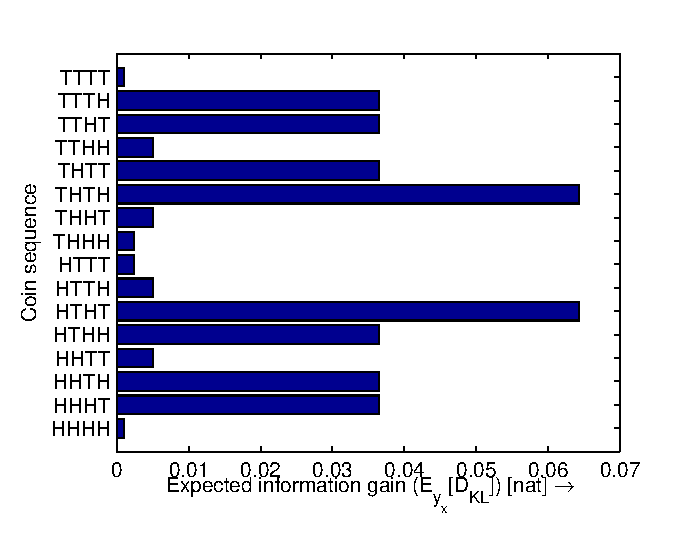
\includegraphics[width=3in]{img/coin.eps}
\caption{Running OED in the subjective randomness domain}
\lou{make this figure in ggplot, clean it up}
\label{fig:run-coin}
\end{figure}

We see that \lstinline{HTHT} and \lstinline{THTH} are the most informative experiments.
Inuitively, this is sensible -- the weighted model infers a 0.5 probability of heads and so assigns equal probability of heads and tails to the next flip, whereas the Markov infers that the probability of transitioning from one outcome to the other is quite high and assigns high probability to the opposite of the last observed value (\lstinline{T} for \lstinline{THTH} and \lstinline{H} for \lstinline{HTHT}).

We also see that \lstinline{HHHH} and \lstinline{TTTT} are the least informative experiments.
Informally, this is because the models make the same predictions for these experiments.
For instance, for \lstinline{HHHH}, the weighted model infers a high probability of heads and so assigns high probability of heads to the next flip.
The Markov model infers a low probability of transitioning from heads to tails, so it also assigns a high probability of heads to the next flip.

\subsection{Experiments?}


\section{Case study 2: Category learning}

\lou{rewrite this paragraph}
We now consider a richer example in the domain of category learning.
The ability to form concepts and abstract rules is an integral component of cognitive science as it establishes a foundation for naming objects and events, as well as discussing and interacting with them.
Since few concepts are formally taught, the formation and progression of classifying observations and experience into categories must be a fundamental learning phenomenon.
As such, models of classification learning has been an active area of research in cognitive science for decades~\cite{machery10:bbs}.

This case study builds on a classic paper by Medin and Schaffer~\cite{medin78:pr}, who considered two competing models of category learning -- the so-called \emph{exemplar model} and the \emph{prototype model} -- and sought to distinguish them by running a cleverly designed experiment.
Medin and Schaffer found that the exemplar model better fit the results of this experiment, so they concluded that it was a better model of human category learning.

Here, we ask: from an information-theoretic perspective, how good was the experiment that Medin and Schaffer designed?
Using OED, we find that there are many superior experiments that Medin and Schaffer could have designed but did not.\footnote{Our work here is an exercise in counterfactual history; the exemplar and prototype models, as expressed in the Medin and Schaffer work, are not state of the art models. We chose the Medin and Schaffer research (rather than newer work) as an object of study because it commits to a clear set of competing models and a clear and tractable set of possible experiments.}

%\lou{worth noting that having oed allows us to determine information-theoretic value of the MS experiment.}

% and illustrates how automated experiment design can outperform human intuition. In particular, this case study demonstrates the efficacy of OED in psychology for discrete and non-ordinal experiment spaces, large combinatoric experiment spaces, and parametric model classes.

\subsection{Models}

\cas{both models are classifiers that take as input an object (a vector of boolean features) and return as output a probability distribution on a/b categorization}

\cas{exemplar model assumes that people store information about every exemplar they've seen and that categorization of an object is a function of similarity to all A exemplars versus B exemplars}

\begin{lstlisting}[caption=Exemplar model (TODO: clearer input/output types)]
var exemplar = function(as, bs) {
  var weights = repeat(4, function() { uniform(0,5) })
  Enumerate(function() {
    var object = repeat(4, function() { flip() ? 1 : 0});
    var sim = function(x,y) {
      product(map3(
         function(xi,yi, wi) { (xi == yi) ? 1 : wi },
         x, y, weights))
    };
    var aSims = sum(map(function(a) { return sim(object, a) }, as));
    var bSims = sum(map(function(b) { return sim(object, b) }, bs));
    condition(flip(ssa / (ssa + ssb)));
    return {object: object, prob: prob}
  })
}
\end{lstlisting}

\cas{prototype model assumes roughly that people do not store every exemplar but instead store something like a prototype for each category and that categorization of an object is a function of its similarity the prototypes (this model produces rank orderings but we did a transform so that it gives numbers)}

\begin{lstlisting}[caption=Prototype model]
var prototype = function(as, bs) {
  var alpha = TODO();
  var bias = TODO();
  var weights = TODO();
  var recall = append(as,bs);
  Enumerate(function() {
    var object = repeat(4, function() { flip() ? 1 : 0});

    var dimEvidenceForA = function(i) {
      var matchingObjects = filter(function(x) { x[i] == object[i] }, recall);
      var n = matchingObjects.length;
      var matchingAs = filter(function(x) { contains(as, x) }, matchingObjects);
      var nA = matchingAs.length;
      var nB = n - nA;
      return weights[i] * (nA - nB)/n;
    }

    var totalEvidence = sum(map(dimEvidenceForA,[0,1,2,3])) + (contains(recall, object) ? bias : 0);

    // TODO: use bias argument
    var prob = 1 / (1 + exp(-alpha * totalEvidence));
    condition(flip(prob));

    return {object: object, prob: prob};
  })
}
\end{lstlisting}

\subsection{Experiments}

\cas{4 binary dimensions - 16 objects total}

\cas{constraints: 9 training stimuli (5 A's and 4 B's)}

\cas{measure: recall and transfer}

\subsection{Results of optimal experimental design}

\cas{we enumerated the 933 valid and unique (up to permuting the dimensions) experiments in terms of expected information gain.}

\cas{we found that the MS experiment was not the best. TODO: reproduce daniel's results (Fig.~\ref{fig:dist})}

\cas{the optimal experiment that we found was TODO}

\begin{figure}[h!]
\centering
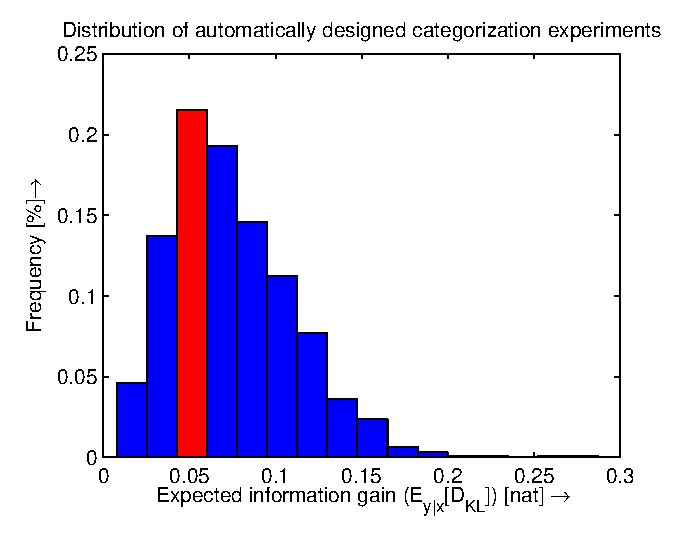
\includegraphics[width=3.2in]{img/dist.eps}
\caption{The distribution of optimal experiments with the MS bin highlighted in red. TODO: add predictions of MS and opt experiment}
\label{fig:dist}
\end{figure}

The MS uses a qualitative swap in ranking for two stimuli to disambiguate the models.
However, this prediction has a relatively small magnitude and comes at the expense of little information gain from the remaining stimuli.
The optimal experiment is better able to quantitatively disambiguate the models by maximizing the information from all the stimuli simultaneously
\lou{note that the OED framework is quite flexible. in our model space, we can also encode hard constraints like ``the models must predict different rank orderings''}

\cas{we conducted the actual experiments. empirical information gain from MS was TODO, empirical information gain from opt was TODO.}

\cas{explain different scales for theoretical versus empirical information gain}

\section{Relationship to previous work}
\section{Discussion}

The purpose of \red{our(?)} OED approach is to quantify the ability of an experiment to differentiate competing computational models. Our approach leverages Bayesian inference to reason about which model best describes a given phenomenon. By using the models' predictions to compute the likelihood of observing a particular response to an experiment, this approach provides a rational method for updating the change in belief about model uncertainty when such responses are observed. This change in belief is then quantified using information theoretic measures, and by maximizing these measures, OED allows one to find experiments that should maximally change the uncertainty of the beliefs in our models.


In this paper, we focus our analysis on the OED criteria of expected KL divergence and its properties, as opposed to the argument of the maximum component of the expression. \ndg{?} The reason is that Eq.~\ref{eq:oed} can rarely be solved analytically and solving it numerically is often a daunting task. To illustrate the advantages of our OED approach, we will be exhaustively evaluating the expected KL divergence for the entire  space of experimental prompts. This allows us to obtain a comprehensive analysis of the entire design space, and the challenge of selecting the optimal experiment is reduced to a simple sorting task. For large design spaces where exhaustive search is intractable, numerical optimization approaches, such as Sequential Monte Carlo searches (REF) or Bayesian optimization (REF), are viable options.  \ndg{move this to dicussion?}



\lou{say some stuff about OED for non-psych experiments}

\bibliographystyle{ieeetr}
\bibliography{oed_nips_2016}

\end{document}
